\section{OpAmp}
\subsection{Realer OpAmp}
    \begin{table}[H]
        \begin{tabular}{l l r r}
            \toprule
            Symbol & Erklärung & Ideal & Real \\
            \midrule
            \(V_0\) & Verstärkung & \(\infty\) & \(10^5..10^8\) \\
            \(V_{Gl}\) & Gleichtaktvers. & \(0\) & \(0,1..0,3\) \\
            \(r_E\) & AC Eingangs-R & \(\infty\) & \(10^7..10^12 \mathrm{\Omega}\) \\
            \(r_{gl}\) & DC Eingangs-R & \(\infty\) & \(r_{gl} > r_E\) \\
            \(I_{P0}, I_{N0}\) & Eingangsstrom & \(0\) & \(0,1..25 \mathrm{nA}\) \\
            Slew Rate &  & \(\infty\) & \(0,5..1000 \mathrm{\frac{V}{\mu s}}\) \\
            \(U_{D0}\) & Offsetspannung & \(0\) & \(0,1..5 \mathrm{mV}\) \\
            \bottomrule
        \end{tabular}
    \end{table}

    \vspace{-16pt}

    \begin{gather*}
        I_{P0} = I_{B+} \quad I_{N0} = I_{B-} \\
        I_B = \frac{I_{B+} + I_{B-}}{2} \\
        I_{OS} = I_{B+} - I_{B-}
    \end{gather*}

\subsection{Grundschaltungen}

    \subsubsection{Invertierender Verstärker}
        \noindent
        \begin{minipage}{0.5\columnwidth}
            \centering
            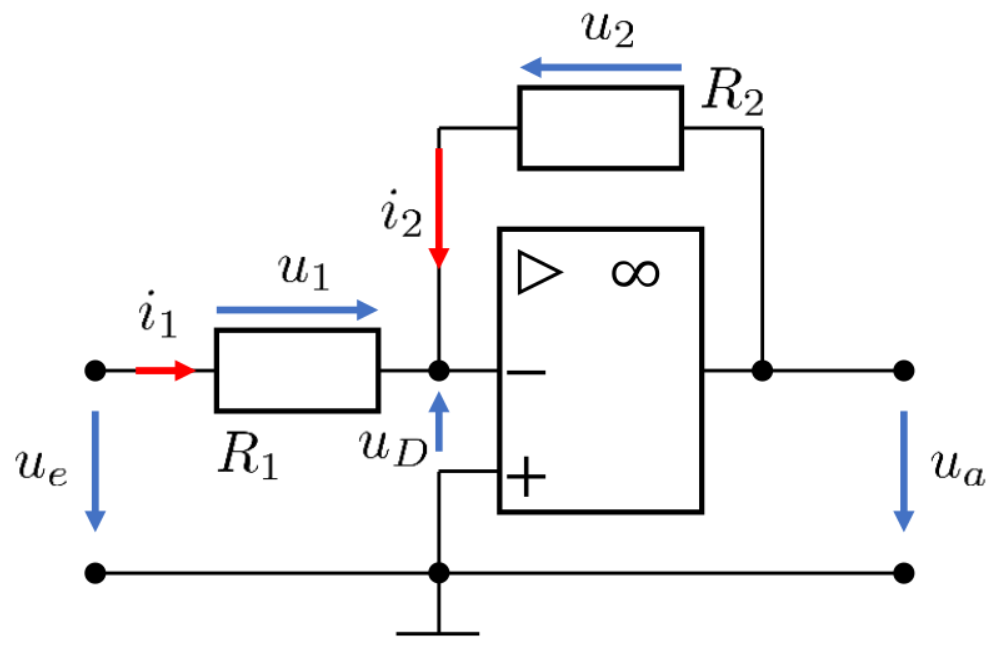
\includegraphics[width=\linewidth]{Figures/opamp/invertingamp.png}
        \end{minipage}%
        \hfill
        \begin{minipage}{0.45\columnwidth}
            \begin{flalign*}
                & u_a = - \frac{R_2}{R_1} \cdot u_e &
            \end{flalign*}
        \end{minipage}
        \vspace{10pt}
    
    \subsubsection{Nicht-Invertierender Verstärker}
        \noindent
        \begin{minipage}{0.5\columnwidth}
            \centering
            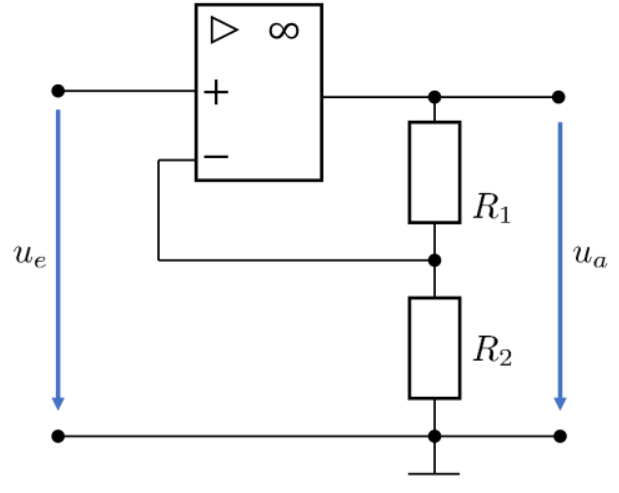
\includegraphics[width=\linewidth]{Figures/opamp/noninvertingamp.png}
        \end{minipage}%
        \hfill
        \begin{minipage}{0.45\columnwidth}
            \begin{flalign*}
                & u_a = \left(1 + \frac{R_1}{R_2} \right) \cdot u_e &
            \end{flalign*}
        \end{minipage}
        \vspace{10pt}

    \subsubsection{Invertierender Addierer}
        \vspace{-10pt}
        \begin{figure}[H]
            \centering
            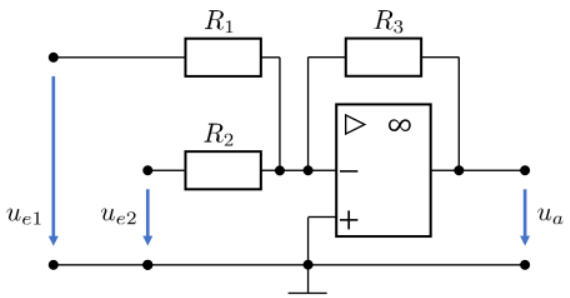
\includegraphics[width=0.6\columnwidth]{Figures/opamp/invertingadder.png}
        \end{figure}
        \vspace{-10pt}
        \begin{align*}
            u_a = - R_3 \cdot \left(\frac{u_{e1}}{R_1} + \frac{u_{e2}}{R_2} \right)
        \end{align*}

    \subsubsection{Subtrahierer}
        \vspace{-10pt}
        \begin{figure}[H]
            \centering
            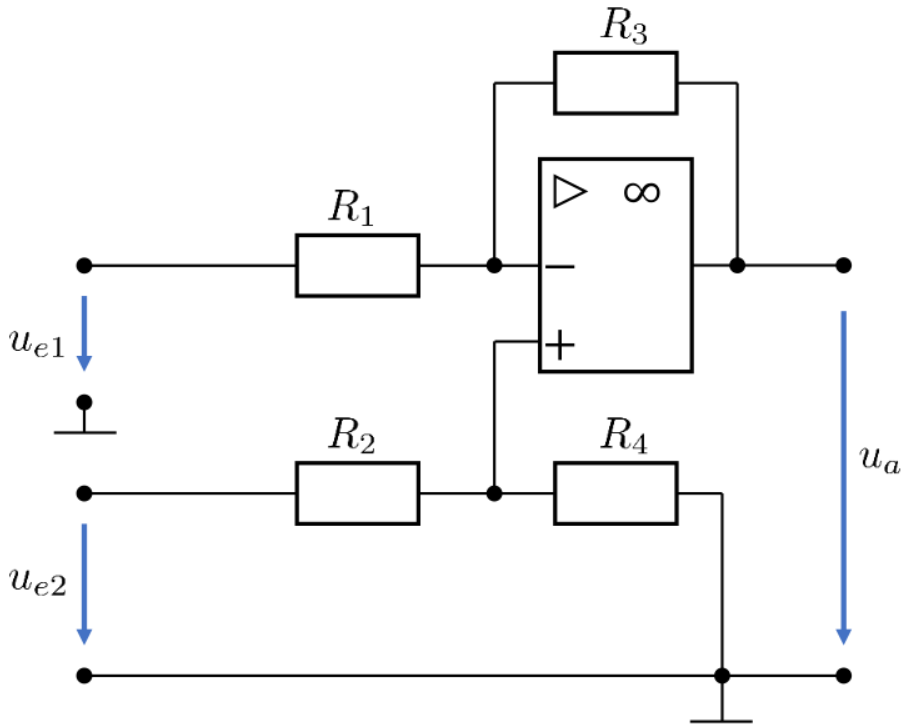
\includegraphics[width=0.6\columnwidth]{Figures/opamp/subtractor.png}
        \end{figure}
        \vspace{-10pt}
        \begin{align*}
                u_a &= \frac{R_4 (R_1 + R_3)}{R_1 (R_2 + R_4)} u_{e2} - \frac{R_3}{R_1} u_{e1} \\
                u_a &= \frac{R_3}{R_1} (u_{e2} - u_{e1}) \qquad \text{wenn} \quad \frac{R_1}{R_3} = \frac{R_2}{R_4}
        \end{align*}

        \textbf{Alternative 1: }
        \vspace{-10pt}
        \begin{figure}[H]
            \centering
            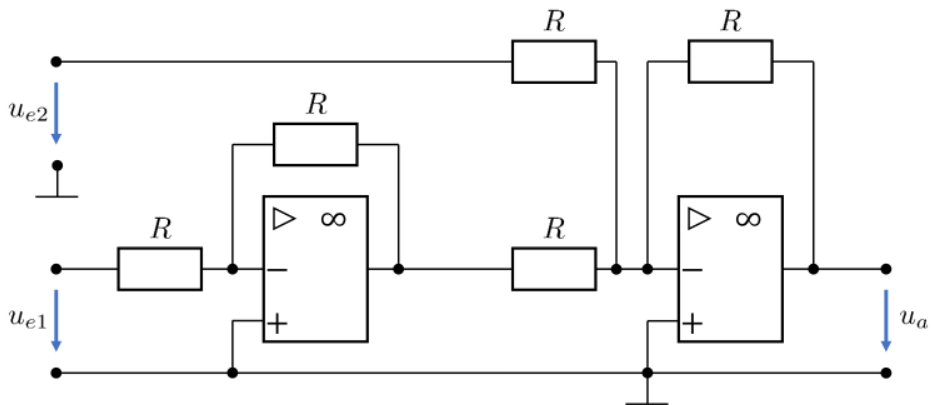
\includegraphics[width=0.7\columnwidth]{Figures/opamp/subtractor_alternative.png}
        \end{figure}
        \vspace{-10pt}
        Aufbau aus Invertierer + Invertierender Addierer
        \begin{align*}
            & u_a = u_{e1} - u_{e2} &
        \end{align*}

        \textbf{Alternative 2: }\\
        \noindent
        \begin{minipage}{0.4\columnwidth}
            \centering
            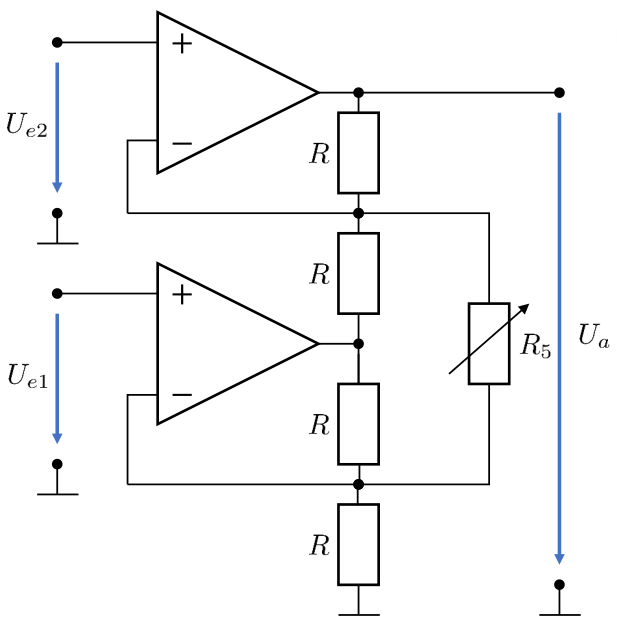
\includegraphics[width=\linewidth]{Figures/opamp/subtractor_alternative2.png}
        \end{minipage}%
        \hfill
        \begin{minipage}{0.55\columnwidth}
            \raggedright
            \begin{flalign*}
                & u_a = 2 \cdot \left( 1 + \frac{R}{R_5} (u_{e2} - u_{e1}) \right) &
            \end{flalign*}
            {\small Vorteil: Nur ein Widerstand zur Einstellung der Verstärkung}
        \end{minipage}
        \vspace{10pt}

    \subsubsection{Integrierer}
        \noindent
        \begin{minipage}{0.4\columnwidth}
            \centering
            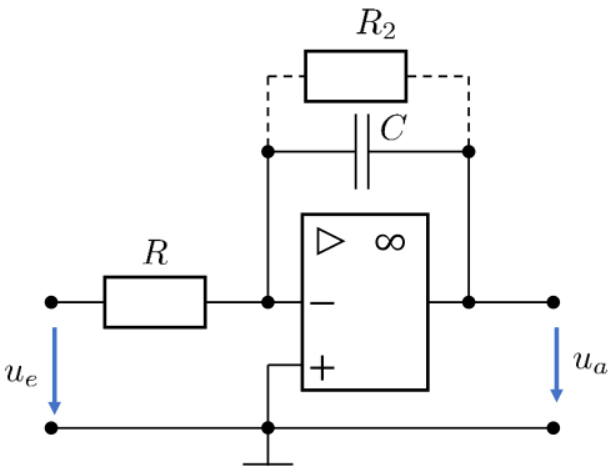
\includegraphics[width=\linewidth]{Figures/opamp/integrator.png}
        \end{minipage}%
        \hfill
        \begin{minipage}{0.55\columnwidth}
            \begin{flalign*}
                & u_a = - \frac{1}{RC} \int_{0}^{t} u_e(t) dt + u_a(0) &
            \end{flalign*}
        \end{minipage}
        \vspace{15pt}

        \textbf{Spezialfall: Ladungsverstärker} (\(R = 0\))\\
        \noindent
        \begin{minipage}{0.45\columnwidth}
            \centering
            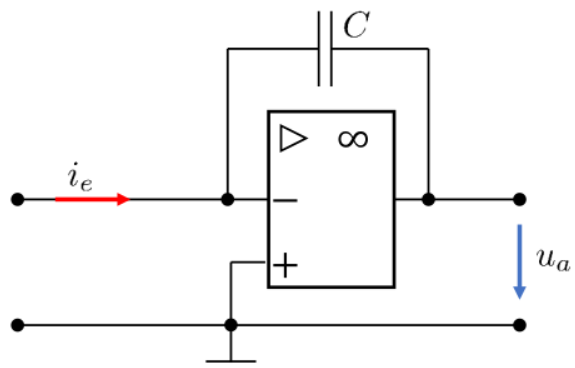
\includegraphics[width=\linewidth]{Figures/opamp/chargeamp.png}
        \end{minipage}%
        \hfill
        \begin{minipage}{0.55\columnwidth}
            \begin{flalign*}
                & \begin{aligned}
                    u_a &= - \frac{1}{C} \int_{0}^{t} i_e(t) dt + u_a(0) \\
                        &= \frac{-q(t)}{C} + u_a(0)
                \end{aligned} &
            \end{flalign*}
        \end{minipage}
        \vspace{10pt}

    \subsubsection{Differenzierer}
        \noindent
        \begin{minipage}{0.4\columnwidth}
            \centering
            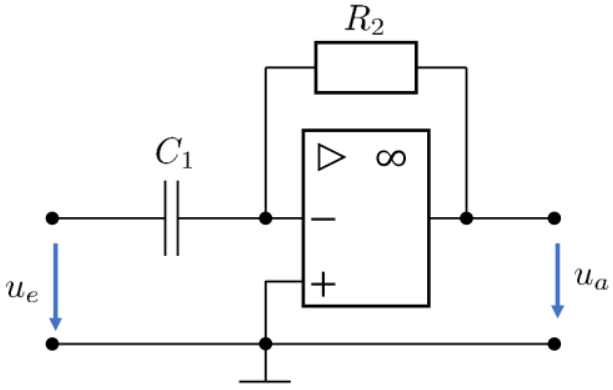
\includegraphics[width=\linewidth]{Figures/opamp/differentiator.png}
        \end{minipage}%
        \hfill
        \begin{minipage}{0.55\columnwidth}
            \raggedright
            \begin{flalign*}
                & U_a (\omega) = - j \omega \cdot R_2 C_1 \cdot U_e(\omega) &
            \end{flalign*}
            \small Schaltung neigt stark zum Schwingen.
        \end{minipage}
        \vspace{15pt}

        \textrightarrow \textbf{Realisierung} (D + PT2-Glied)\\
        \vspace{-10pt}
        \begin{figure}[H]
            \centering
            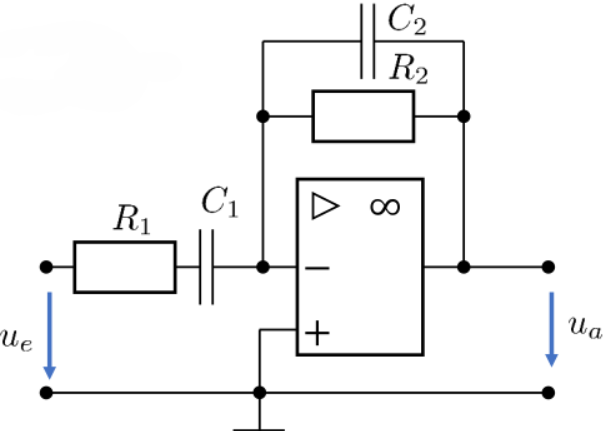
\includegraphics[width=0.5\columnwidth]{Figures/opamp/differentiator_real.png}
        \end{figure}
        \vspace{-10pt}
        \begin{align*}
            & U_a (\omega) =  \frac{ - j \omega \cdot R_2 C_1 \cdot U_e(\omega) }{(1 + j \omega R_1 C_1) \cdot (1 + j \omega R_2 C_2)} &
        \end{align*}

    \subsubsection{Transistor im Rückkopplungspfad}

    